\section{Results}
\label{sec:experiments}

\subsection{Experimental Setup}

\paragraph{Datasets and tasks.}
For all our experiments,
we use datasets and tasks from RelBench~\citep{relbench,gu2026relbenchv2}.
RelBench v1 contains $7$ relational databases from diverse domains, namely,
\texttt{rel-amazon}, \texttt{rel-hm}, \texttt{rel-stack},
\texttt{rel-avito}, \texttt{rel-event}, \texttt{rel-trial} and \texttt{rel-f1}.
Each dataset has multiple forecasting tasks defined on it,
which are either binary classification or regression.
For example, for \texttt{rel-amazon},
there are $4$ forecasting tasks
(\texttt{user-churn}, \texttt{item-churn}, \texttt{user-ltv} and \texttt{item-ltv}),
of which the first $2$ are binary classification,
and the last $2$ are regression.
We also define autocomplete tasks,
both binary classification and regression,
on all datasets
(App.~\ref{app:autocomplete_tasks}).
See App.~\ref{app:relbench_suitability} for detailed characteristics
which make RelBench suitable for pretraining and evaluation.

RelBench provides standardized temporal splits for tasks,
as well as cutoff timestamps for the databases.
We pretrain and fine-tune only on the training splits of the tasks,
using database rows only up to the training cutoff timestamps.
To pick the best checkpoints,
we use the validation task splits and
validation cutoff timestamps.
We report the test set performance,
for both learning curves and tables.
We evaluate only on the forecasting tasks,
as autocomplete tasks are not part of the standard RelBench benchmark.
We skip \texttt{rel-event},
as it has been found to have temporal leakage issues.

\paragraph{Leave-one-DB-out pretraining.}
The strongest setting to demonstrate transfer is
when both the dataset and task are unseen.
We expect cross-dataset transfer despite disparate application domains as
databases share structural commonalities, e.g.,
dimension tables, fact tables, hubs and tripartite structures~\citep{relgnn},
as well as semantic similarities, e.g.,
similar user behaviors
when
reviewing books (\texttt{rel-amazon}),
commenting on posts (\texttt{rel-stack}),
attending events (\texttt{rel-event}),
purchasing clothes (\texttt{rel-hm}),
and clicking on ads (\texttt{rel-avito}),
which RT could learn to identify and exploit.
Due to the limited number of different databases,
we pretrain separately for each target dataset
on all tasks from all other datasets.
We select the best validation checkpoint~\citep{ranjan2024post}
separately for each target task as
we found significant overfitting during pretraining
due to limited pretraining tasks.
% However, regularization or recommendations from~\cite{ranjan2024post}
% didn't help suggesting different overfitting dynamics than in
% supervised learning settings.


% Due to limited number of different databases,
% we pretrain and evaluate models in a \textit{leave-one-DB-out} manner.
% For example, let \texttt{rel-amazon} be the held-out dataset.
% We pretrain on all forecasting and autocomplete tasks from the other $6$ datasets,
% namely,
% \texttt{rel-hm}, \texttt{rel-stack},
% \texttt{rel-avito}, \texttt{rel-event}, \texttt{rel-trial} and \texttt{rel-f1}.
% Among the checkpoints obtained during this pretraining run,
% we pick the best one for each forecasting task from \texttt{rel-amazon}
% namely,
% \texttt{user-churn}, \texttt{item-churn}, \texttt{user-ltv} and \texttt{item-ltv},
% based on the zero-shot performance on the validation set of that task.
% Thus, for all experiments,
% the target dataset and task is unseen during pretraining,
% except to the extent of model selection
% based on zero-shot validation performance.

% In this setup,
% the pretrained model has never seen any task associated with the dataset
% for which the downstream task is defined,
% or even its schema.
% This is the strongest setting to test for transfer learning.

% \rr{should intuition to expect transfer be in intro?}
% \mf{it is unclear to a reader why this is expected to work, and I don't find a good answer yet in the paper. What patterns can we expect to learn on Amazon and H\&M that can then be applied to F1?}

% Note that even though some tasks have similar names,
% e.g. \texttt{rel-amazon/user-churn} and \texttt{rel-hm/user-churn},
% they are very dissimilar distributionally.
% For example, \texttt{rel-amazon} is about reviewing books on Amazon,
% whereas \texttt{rel-hm} is about purchasing clothes on H\&M,
% and both have distinct schemas.
% Moreover, \texttt{user-churn} needs to be predicted over a 3 month period
% for \texttt{rel-amazon}, but over a $7$ day period for \texttt{rel-hm}.

\paragraph{Architecture details.}
We use a $12$ layer transformer
with hidden dimension $256$ and
$8$ attention heads per layer.
We use gated MLPs with SiLU activation,
as found in the LLaMA architecture \citep{llama},
with hidden dimension $1024$.
For text embeddings,
we use the MiniLMv2~\citep{minilmv2} model
from SentenceTransformers~\citep{sentence_transformers},
which produces $384$ dimensional embeddings.
With this configuration,
the architecture has about $22$M trainable parameters.

\paragraph{Training details.}
We pretrain RT for $50$k steps
at a context length of $1024$,
with a batch size of $256$,
AdamW optimizer with weight decay $0.1$,
and a peak learning rate of $10^{-3}$,
with linear warmup from zero for the first $20\%$ of training,
and linear decay to zero for the remainder.
On each downstream task,
we fine-tune for $33$k steps
with the same context length, batch size and optimizer as above,
but with a constant learning rate of $10^{-4}$
and no weight decay.
One pretraining (fine-tuning) run takes
around $2$ hours ($1.5$ hours) on $8\times$A100 GPUs at BFloat16 precision,
with a training throughput of around $8$ batches/second or $2$M tokens/second.


\paragraph{Baselines.}
We compare RT against schema-agnostic methods,
which can be pre-trained on diverse databases,
and schema-specific ones,
which cannot. Schema-agnostic baselines include \textbf{Griffin}~\citep{griffin}, pretrained and fine-tuned with the same setup as RT and matched in parameter count, and \textbf{LLM}, where we prompt Gemma3~\citep{gemma3} models with instructions followed by a text-serialized database subgraph identical to that used for RT~\citep{snowflake2024relational}. Schema-specific baselines include \textbf{RDL-GNN}~\citep{relbench}, which encodes rows into node vectors via tabular encoders and aggregates across tables with GNN layers, \textbf{RelLLM}~\citep{relllm}, which combines GNN encoders with LLMs in a retrieval-augmented framework, \textbf{RelGNN}~\citep{relgnn} and \textbf{RelGT}~\citep{relgt} (latter $2$ are in App.~\ref{app:finetuning}).
The non-neural \textbf{EntityMean} baseline predicts the mean of the past labels for the target entity. See App.~\ref{app:baselines} for more details.

% \subsubsection{Schema-agnostic}
% These baselines can be pretrained
% and evaluated for zero-shot transfer on unseen datasets.
% \textbf{Griffin ~\cite{griffin}.}
% We compare against Griffin as an alternative architecture.
% Hence, Griffin is pretrained/fine-tuned with the same data and setup as RT.
% Further, we pick hyperparameters for Griffin such that it has the same
% number of parameters as RT.




% \textbf{RelLLM ~\cite{relllm}.} RelLLM combines GNN encoders with LLMs in a retrieval augmented generation framework.

% \textbf{LLM.}
% We prompt Gemma3~\citep{gemma3} models of various sizes with instructions/descriptions
% followed by a text-serialized database subgraph.
% The subgraph is exactly identical to what we use for RT,
% and the text-serialization is borrowed from \citet{snowflake2024relational}.
% See App.~\ref{app:llm_prompting} for details.

% \subsubsection{Schema-specific}
% These baselines have parameters tied to specific tables and columns,
% and can only be used for dataset- and task-specific supervised learning.

% \textbf{RDL-GNN~\citep{relbench}.}
% RDL-GNN is the first architecture capable of
% end-to-end relational deep learning (RDL).
% It consists of tabular encoder layers
% to encode rows into node vectors,
% followed by graph neural network (GNN) layers
% to aggregate information across tables.
% We make some improvements for regression tasks (App.~\ref{app:gnn_improvements}).

% \textbf{RelGNN~\cite{relgnn}.} RelGNN introduces a composite message passing mechanism to address structural inefficiencies of existing heterogeneous GNNs for relational databases.

% \textbf{RelGT~\cite{relgt}.} The Relational Graph Transformer is a graph-transformer architecture tailored to relational databases. RelGT utilizes a specialized tokenization approach to efficiently encode heterogeneity, temporality, and topology of the graph. It then pairs local attention on sampled subgraphs with global attention to a small set of learnable centroids, unifying local and database-wide information.



\subsection{Learning Efficiency}

The key promise of pretraining is
efficient adaptation to new datasets and tasks.
Adaptation can be via zero-shot prompting,
few-shot learning or fine-tuning.
Since we pretrain only on a handful of different databases,
we focus on efficient fine-tuning in this work.
Remarkably, we see the \textbf{emergence of zero-shot abilities} in RT,
which we compare with relevant baselines in \S~\ref{sec:zero_shot}.

% In particular,
% we are interested in fine-tuning on downstream tasks
% only for a few steps.
% This is important in practice,
% because fine-tuning is data- and compute-intensive,
% both of which are in a premium in many applications.
% With enough fine-tuning,
% it is expected that untrained models
% can catch up with pretrained models.


\begin{figure} [t]
\centering
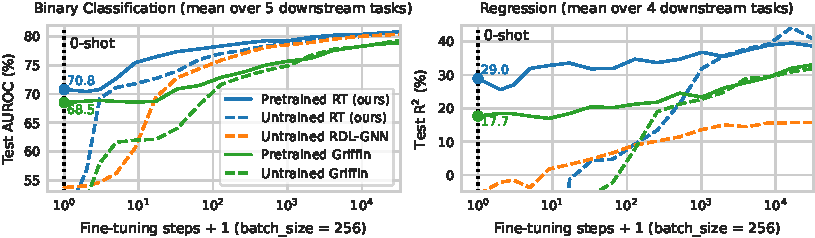
\includegraphics{auto-figures/learn-avg.pdf}
\caption{
Test set learning curves up to 32k fine-tuning steps
(8M training examples, including repetitions).
Averaging is done over tasks which do not show overfitting.
X-axis is on log-scale.
The first point on each curve is the zero-shot performance.
Target datasets and tasks are unseen during pretraining.
Pretraining data is the same for both RT and Griffin.
Pretrained RT is best overall,
and untrained RT catches up towards the end.
}
\label{fig:learn-avg}
\end{figure}

\paragraph{Setup.}
In Fig.~\ref{fig:learn-avg},
we show learning curves for supervised fine-tuning
on downstream tasks for
RT (pretrained and untrained),
RDL-GNN (untrained),
and Griffin (pretrained and untrained).
We average the curves over tasks which do not show overfitting.
For all these models,
we use the same fine-tuning setup as described above.
Full fine-tuning results for all tasks,
are in App.~\ref{app:finetuning}

\paragraph{Observations.}
% 1)
Our first observation is that RT exhibits strong zero-shot performance, demonstrating effective transfer from pretraining to unseen databases and tasks.
While Griffin also benefits from zero-shot transfer, 
% when adapted to treat task tables as additional database tables, 
RT consistently outperforms it.
% 2)
The pretrained RT consistently maintains the gap in performance based on its strong initialization and is only caught up by the untrained RT and RDL-GNN on classification tasks after extensive fine-tuning.
% 3)
Notably, fine-tuning from a pretrained checkpoint shows a small dip in performance in the very early steps, which we conjecture might be due to the model transitioning from a zero-shot, in-context-labels- and semantics-driven regime to a data-driven prediction regime.
% 4)
Finally, while RDL-GNN initializes faster than untrained RT, the latter overtakes it after a few training steps ($2$ on classification and $\approx100$ on regression).

\begin{table}[t]
\CatchFileDef{\data}{auto-tables/zs-auc.tex}{}
\centering
\scriptsize
\begin{tabular}{llrrrrrrrrr}
\toprule
\multicolumn{2}{r}{Target DB $\in$ pretraining? $\rightarrow$}
& \multicolumn{3}{c}{Maybe}
& \multicolumn{3}{c}{No}
& \multicolumn{3}{c}{Yes}
\\
\cmidrule(lr){3-5} \cmidrule(lr){6-8} \cmidrule(lr){9-11}
Dataset $\downarrow$
& Task $\downarrow$
& Gemma
& Gemma
& Gemma
& \makecell{Entity\\Mean}
& Griffin
& \makecell{RT\\(ours)}
& \makecell{Rel\\LLM}
& Griffin
& \makecell{RT\\(ours)}\\
\cmidrule{1-11}
\multicolumn{2}{r}{Parameter count $\rightarrow$}
& 4B
& 12B
& 27B
& 0
& 22M
& 22M
& 3B
& 22M
& 22M \\
\midrule
\data
\bottomrule
\end{tabular}
\caption{
Zero-shot test AUROC (\%) for $10$ binary classification tasks.
Higher is better.
Random/majority baseline is $50.0$.
For RelLLM we use their own prompt construction.
Other baselines have equivalent database subgraphs.
Gemma and RelLLM additionally include dataset and task descriptions,
as well as natural language instructions.
The target task is never seen during pretraining.
}
\label{tab:zero-shot-clf}
\end{table}





\subsection{Zero-Shot Prompting}
\label{sec:zero_shot}

\paragraph{Setup.}
In Tabs.~\ref{tab:zero-shot-clf} and \ref{tab:zero-shot-reg-no-llm},
we report zero-shot results.
The target task is always unseen.
We report results for when the target dataset is also unseen,
as well as after doing some continued pretraining on the target dataset.
\rev{Columns ``No'' and ``Yes'' respectively in Tabs.~\ref{tab:zero-shot-clf}, \ref{tab:zero-shot-reg-no-llm}).
Pretraining data for Gemma models is unknown,
but likely includes similar public datasets (e.g., F1, Amazon and StackExchange),
hence they are grouped under ``Maybe''.
}
For RT and Gemma, we construct the input context using our sampling algorithm.
For Griffin, we adapt its sampling procedure to include rows from task tables, making it consistent with our task table prompting to enable zero-shot capabilities.
For RelLLM we use their own prompt construction. 
Both RelLLM and Gemma baselines are additionally provided with textual task descriptions and instructions.
% We include a simple but effective baseline by averaging past target entity labels that appear in the sampled subgraph (\textit{Entity Mean}). 


\begin{table}[t]
\CatchFileDef{\dataClf}{auto-tables/enc-auc.tex}{}
\CatchFileDef{\dataReg}{auto-tables/enc-r2.tex}{}
\CatchFileDef{\data}{auto-tables/zs-r2-no-llm.tex}{}
\centering
\begin{minipage}[b]{0.54\textwidth}
\centering
\scriptsize
\setlength{\tabcolsep}{3pt}
\begin{tabular}{llrrrrr}
\toprule
\multicolumn{2}{r}{Target dataset $\in$ pretraining? $\rightarrow$}
& \multicolumn{3}{c}{No}
& \multicolumn{2}{c}{Yes}
\\
\cmidrule(r){3-5} \cmidrule{6-7}
Dataset $\downarrow$
& Task $\downarrow$
& \makecell{Entity\\Mean}
% & Griffin
& Grif.
& \makecell{RT\\(ours)}
% & Griffin
& Grif.
& \makecell{RT\\(ours)}\\
\midrule
\data
\bottomrule
\end{tabular}
\caption{
Zero-shot test R$^2$ (\%) for $8$ regression tasks.
Higher is better.
Global mean baseline is $0.0$.
Setup is same as Table~\ref{tab:zero-shot-clf}.
LLM baselines are poor (App.~\ref{app:llm_poor_regression}).
}
\label{tab:zero-shot-reg-no-llm}
\end{minipage}
\hfill
\begin{minipage}[b]{0.42\textwidth}
\centering
\scriptsize
\setlength{\tabcolsep}{3pt}
\rev{
\begin{tabular}{llrrrr}
\toprule
Dataset $\downarrow$
& Task $\downarrow$
& \multicolumn{3}{c}{MLP-only FT}
& \multirow{2}{*}{\makecell{Full\\FT\\(RT)}} \\
\cmidrule{3-5}
\multicolumn{2}{r}{Embedder (frozen) $\rightarrow$}
% & \makecell{Untrained\\RDL-GNN}
% & \makecell{Untrained\\RT}
% & \makecell{Pretrained\\RT}
& GNN
& RT(U)
& RT(P)
& \\
\midrule
% \multicolumn{6}{l}{
% AUROC (\%) for $5$ binary classification tasks.
% Higher is better.
% % Random/majority baseline is $50.0$.
% } \\
% \cmidrule{1-6}
\dataClf
\midrule
% \multicolumn{6}{l}{
% R$^2$ (\%) for $4$ regression tasks.
% Higher is better.
% % Global-mean baseline is $0.0$.
% } \\
% \cmidrule{1-6}
\dataReg
\bottomrule
\end{tabular}
\caption{
\rev{
RT as feature extractor.
\textbf{GNN, RT(U)} are untrained,
\textbf{RT(P)} is pretrained.}}
\label{tab:enc_ablations}
}
\end{minipage}
\end{table}


\paragraph{Observations.}
% 1)
RT demonstrates non-trivial zero-shot performance on all tasks.
On classification, it attains the best average AUROC and is the only method to consistently beat the entity mean baseline.
On regression, where LLM baselines fail to provide meaningful predictive accuracy, RT is the only model to consistently achieve positive $R^2$
and surpass the EntityMean baseline on average.
% 2)
% These results establish RT as the first architecture capable of robust zero-shot transfer to relational regression tasks, while also achieving state-of-the-art zero-shot performance on relational classification tasks.


\subsection{\rev{Relational Feature Extraction}}
\label{sec:feature_extractor}

\rev{
\paragraph{Setup.}
We use the masked token representation before the decoder layer
from a pretrained RT and fine-tune (FT) only a 2-layer MLP over it
for downstream tasks on unseen datasets.
Results are in Tab.~\ref{tab:enc_ablations},
along with untrained GNN and RT,
as well as full FT for comparison.
}

\rev{
\paragraph{Observations.}
MLP-only FT has $4.3\%$ (abs.) better avg. R$^2$
and only $1.6\%$ (abs.) worse avg. AUROC than full FT,
despite being orders of magnitude cheaper.
Even untrained RT embeddings are sometimes competitive,
and much better than untrained GNN embeddings.
}


\subsection{\rev{Cost-Quality Trade-Off}}
\label{sec:cost_quality}

\begin{figure}[t]
\centering
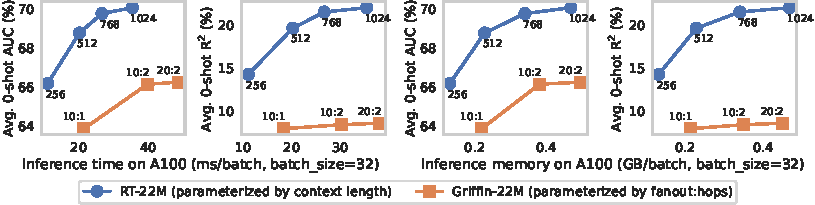
\includegraphics{auto-figures/fig_combined.pdf}
\caption{
\rev{
Cost-quality trade-off w.r.t. varying context sizes at inference.
Pretraining was done at the max context size.
Average is over $10$ classification and $8$ regression tasks.
}
}
\label{fig:combined}
\end{figure}

\rev{
\paragraph{Setup.} Fig.~\ref{fig:combined} shows how zero-shot performance
varies with test-time compute in terms of time and memory.
We vary the context length for RT (a transformer),
and fanout:hops for Griffin (a GNN),
at inference
for models pretrained at max context size---$1024$
for RT, $20$:$2$ for Griffin (default in \citep{griffin}).
}

\rev{
\paragraph{Observations.}
RT dominates Griffin.
This is despite RT being a cell-level transformer,
and Griffin being a row-level GNN, as
(1) FlexAttention kernels used in RT are highly efficient~\citep{flex_attention},
(2) Griffin incurs cell-level penalty in the row encoding step, and,
(3) at equal parameter count and similar context sizes, memory cost is similar.
RT's performance degrades gracefully,
showing a drop of only $4\%$ absolute AUROC and $7\%$ absolute R$^2$
with $25\%$ lower time and $20\%$ lower memory.
}
